\chapter{Introduction}
\label{c.intro}

\section{The Epoch of Reionization}

Our Universe has a complex, rich history, of which enormous progress has been made in the past few decades to unravel its story. Much has been learned about the very beginnings of the Universe, from the Big Bang's large explosion of energy to the relatively smooth and simple cosmic background radiation that was leftover. Additionally, observational feats have revealed the status of the present-day Universe and the intricate \textit{cosmic web}, or large scale structure, of galaxies today. 

The Epoch of Reionization (EoR) ties these two bookends together, occurring about a billion years after the Big Bang when the very first stars and galaxies formed. How did the tiny density fluctuations from the cosmic microwave background develop into the structure we see today? How did the first luminous structures form, and how did they evolve and influence the gas around them? Exploring the reionization era opens up a new chapter of our Universe's story - a chapter that promises to connect the dots between our past and present.

\subsection{Cosmic History}

As the Universe expanded and cooled after the Big Bang, electrons and protons eventually combined to form neutral hydrogen atoms. At the young age of $\sim$ $380,000$ years, the Universe's ordinary baryonic content was almost entirely neutral hydrogen, while most of its total matter was dark matter (\citealt{loeb_furlanetto_2013}). Then, for the next several hundred million years, the \textit{Dark Ages} proceeded, with concentrations of dark matter setting the foundations for the formation of the first luminous structures. More specifically, the tiny, primordial density fluctuations that were established at the release of the CMB grew with inflation and the expansion of the Universe. The densest regions then collapsed to form dark matter halos, inside of which hydrogen gas could cool, condense, and fragment into stars (\citealt{dodelson_cosmology}).

The first luminous structures are thought to have formed at an age of $\sim$ $200$ million years (z $\sim$ 20) and are predicted to have been massive stars with high luminosities and large ionizing powers (\citealt{loeb_furlanetto_2013}). The ionizing photons from the first stars carved out pockets of ionized hydrogen gas around the densest, most massive dark matter halos, and as the number of sources grew, an increased number of ionized bubbles emerged and overlapped. Eventually, the first generations of stars and galaxies succeeded in ionizing most all of the neutral hydrogen in the Universe, with reionization complete by about one billion years after the Big Bang (z $\sim$ 6) (\citealt{furlanetto_et_al2006}). 

\begin{figure}
	\centering
	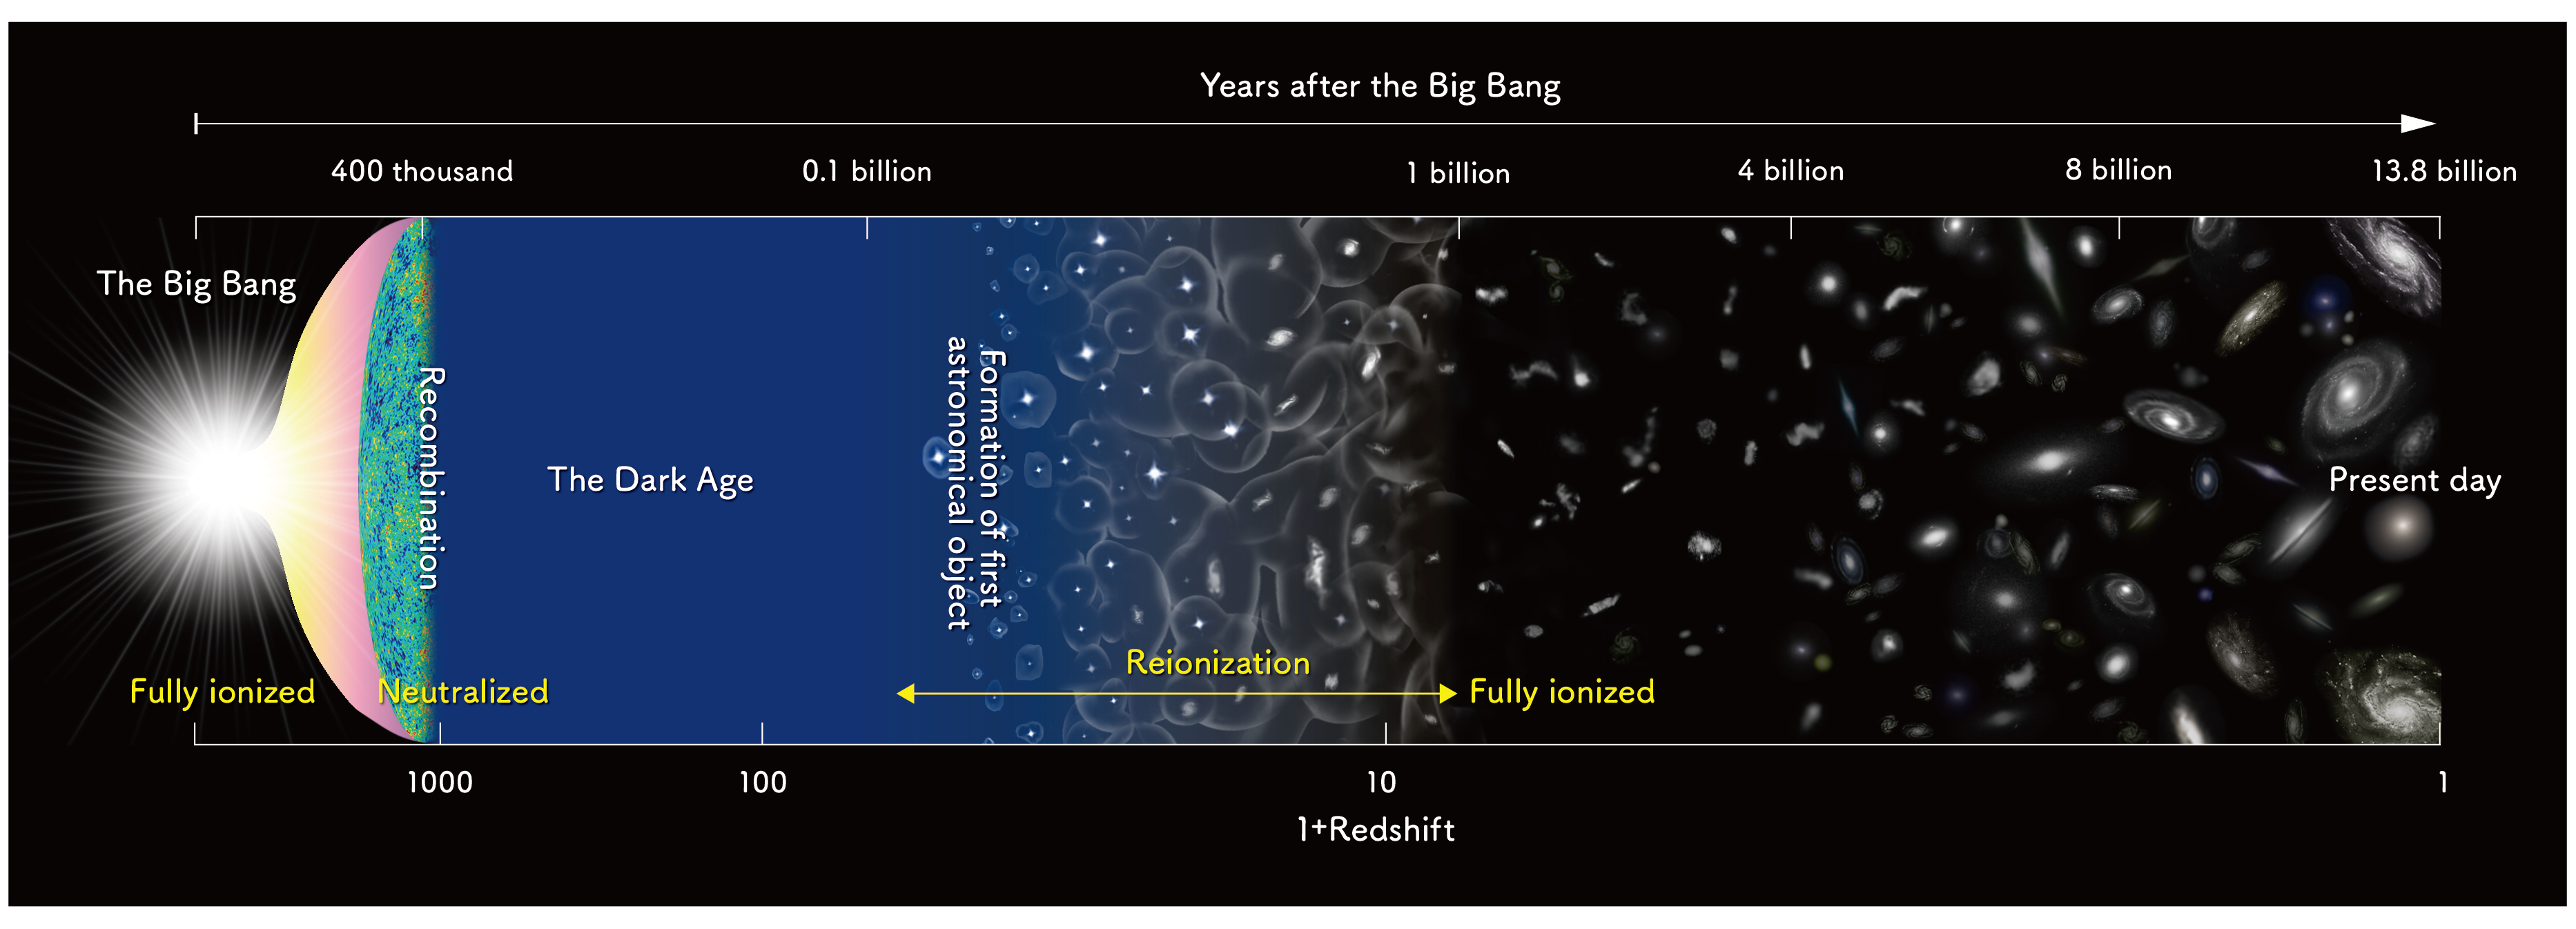
\includegraphics[width=\columnwidth]{plots/timeline_history.jpg}
	\caption{Timeline of the history of the Universe. The Epoch of Reionization marks the era when the first stars and galaxies formed and ionized the neutral hydrogen in the Universe. Image credit: NAOJ.}
	\label{fig:timeline_history}
\end{figure}

The exact timescale and details of the reionization process, which are shown within the context of the history of the Universe in Figure \ref{fig:timeline_history}, are current research questions in the field of cosmology. The physics of reionization depends on several factors, including the nature of the first stars (masses, luminosities, ionizing photons) and the surrounding gas (efficiency of the ionizing photons, feedback effects). Turning the argument around, deep investigations of the reionization era would lead to new understandings about the properties of the first stars and the intergalactic medium (IGM). There are several ways to approach the study of this epoch, with CMB measurements working to constrain the duration of reionization, galaxy measurements unveiling the end of reionization, and direct hydrogen measurements attempting to map out the changing nature of the gas over time. All of these probes serve to illuminate this watershed era between a Universe dominated by darkness and a Universe defined by light.

\subsection{CMB and Galaxy Measurements}

There are several observational probes of the reionization epoch, and we highlight two broad categories in this section. The first is the study of CMB anisotropies, which carry with them an imprint of the early Universe from the time of its release. But that's not the only imprint it has - CMB photons can scatter off of free electrons after reionization, and these scatterings leave behind polarization and temperature imprints (\citealt{haiman_knox_1999}). For example, the amplitude of the CMB is sensitive to scatterings, as an increased number of scatterings is akin to mixing different parts of the CMB together as photons are scattered in all directions. In other words, this scattering washes out anisotropies in the CMB and lowers its overall amplitude. 

A useful parameter to quantify the amount of electron scattering that occurs is the optical depth, $\tau_{es}$, defined as:

\begin{equation}
\tau_{es} = \int n_{e}\sigma_{T} dl,
\end{equation}
where $n_{e}$ is the number density of free electrons, $\sigma_{T}$ is the Thompson cross-section, and the integral is taken over a proper length $dl$. Once reionization begins, the number of free electrons increases, contributing to increasingly higher values of $\tau_{es}$. Hence, an earlier start for reionization would yield higher optical depths than a late reionization scenario. 

Observations of the CMB by WMAP and Planck have placed constraints on the optical depth parameter (\citealt{hinshaw_et_al2013}; \citealt{planck2016}), with the more recent Planck result suggesting a value of $\tau_{es} \sim 0.07$. This value suggests that reionization ends at a redshift of $z \sim 6$, with instantaneous reionization (``mean" reionization) at $z \sim 8.8$ (\citealt{planck2016}).

Currently, the results from CMB measurements are in agreement with a second powerful probe of EoR --- broadly speaking, that of galaxy observations. This probe comes in many flavors. For example, the spectra of distant quasars at high redshifts can illuminate the end of reionization. Quasars, being extraordinarily bright and energetic objects, are detectable at very far distances and their spectra reveal the amount of absorption their light has undergone due to neutral hydrogen. While nearby quasar spectra exhibit sharp absorption lines, distant ones show the Gunn-Peterson trough, implying that the quasar light was entirely suppressed by hydrogen absorption (i.e., neutral hydrogen existed). Studying the absorption features of quasars at different redshifts implies that reionization has indeed ended by $z \sim 6$ (\citealt{becker_et_al2001}). 

In addition to quasar observations, high-redshift galaxy observations can also reveal important characteristics about the state of the IGM. Namely, distant star-forming galaxies can be detected using a variety of techniques, such as narrow-band imaging to find Lyman-$\alpha$ emitters (radiation that is produced by recombination near young stars) or broad-band observations to find Lyman-break galaxies (spectral breaks associated with absorption by neutral hydrogen). High-redshift galaxy observations can then be used to construct luminosity functions (number of stars per luminosity interval) and star formation histories, which in turn impact the evolution of the IGM. 

More specifically, if star-forming galaxies dominated the reionization process, then the ionization rate can be related to the following star-formation parameters:

\begin{equation}
\dot{n}_{\rm ion} = f_{\rm esc}\xi_{\rm ion}\rho_{\rm SFR},
\end{equation}
where $\dot{n}_{\rm ion}$ is the cosmic ionization rate, $f_{\rm esc}$ is the escape fraction of photons into the IGM, $\xi_{\rm ion}$ is the rate of production of ionizing photons for a stellar population, and $\rho_{\rm SFR}$ is the star formation rate density. All three parameters influence the rate at which the IGM is ionized, and the star formation rate density is able to be constructed from galaxy luminosity functions. For example, \citet{robertson_et_al2015} used data from the Hubble Space Telescope to construct a star formation rate history out to high redshifts, backing out an optical depth parameter that is consistent with that of Planck. 

While galaxy measurements can be used to constrain the EoR, they are ultimately doing so by unveiling the properties of old, distant stars and galaxies. A similar, new technique that also aims to reconstruct the histories of the first luminous structures is observing nearby, metal-poor Local Group galaxies. Called ``galactic archaeology," observations of nearby star-forming ancestors can be used to constrain the faint-end slope of the luminosity function. Determining the shape of this function has important implications on the number of galaxies needed to drive reionization and the types of sources dominating this epoch (\citealt{weisz2017}). Additionally, studies of nearby metal-poor stars and galaxies can provide insight into the contents of the first generation of stars and the dynamics of high-redshift star formation, as observations of ultrafaint dwarf galaxies around the Milky Way suggest they are relatively clean tracers of the first generations of stars (\citealt{loeb_furlanetto_2013}).

Galaxy observations for reionization studies have been primarily driven by observations taken by the Hubble Space Telescope. In the coming years, the James Webb Space Telescope (JWST), a 6.5\,m infrared space telescope, will be optimally primed for the detection of faint galaxies, including galaxies whose roots extend as far back as the cosmic dawn and who may exhibit signatures of first generation Population III stars. In addition to JWST, several large infrared ground telescopes are also underway, including the European Extremely Large Telescope (EELT), the Giant Magellan Telescope (GMT), and the Thirty Meter Telescope (TMT). 

Although both CMB measurements and galaxy observations have much to look forward to, they currently each have their limitations. For example, CMB measurements can only reveal the integrated quantity of $\tau_{es}$, therefore unable to provide insight into the evolution of reionization as it progresses over time. Similarly, galaxy observations are currently limited by sensitivity, able to hover only around the tail end of the reionization era. A different, but complimentary, probe is needed to unlock the entire window into the EoR.

\subsection{Measurements of HI}

A direct measurement of neutral hydrogen gas over time would provide a fundamental way to track the IGM over the reionization process. Such a probe, which is made possible by the spin-flip transition of hydrogen, is a powerful technique that allows the tracing of gas over time, and it is this technique that serves as the basis for the remainder of this thesis (\citealt{furlanetto_et_al2006}; \citealt{barkana_and_loeb2008}; \citealt{morales_and_wyithe2010}; \citealt{pritchard_and_loeb2010}; \citealt{pritchard_loeb2012}). 

The spin-flip transition of neutral hydrogen occurs when a hydrogen atom changes energy state between two hyperfine levels. Namely, if a hydrogen atom moves from an aligned energy state (the proton and electron have parallel spins) to an anti-aligned state (the proton and electron have antiparallel spins), the energy difference is released in the form of a photon with a wavelength of $21$\,cm. 

Because this transition has a well-defined wavelength, the signal can be directly mapped to a distance, or redshift, by measuring its wavelength upon detection. For example, a $21$\,cm photon that was initially emitted at a redshift of $z = 6$ would have expanded by a factor of ($1+z$) due to the expansion of the Universe and be $1.5$\,m long when it arrives at our telescopes. Hence, observing longer wavelengths of the hydrogen signal means that it has traveled for a greater distance (and has stretched out more) and thus comes from farther away at a higher redshift. This means that the $21$\,cm signal is a powerful tracer of neutral hydrogen at any distance (i.e., as a function of time), as long as it exists. This technique is especially compelling because it allows the direct exploration of the EoR as reionization occurs, whereas CMB measurements and galaxy measurements surround this era from the beginning and end only, respectively (Figure \ref{fig:timeline_circle}).

\begin{figure}
	\centering
	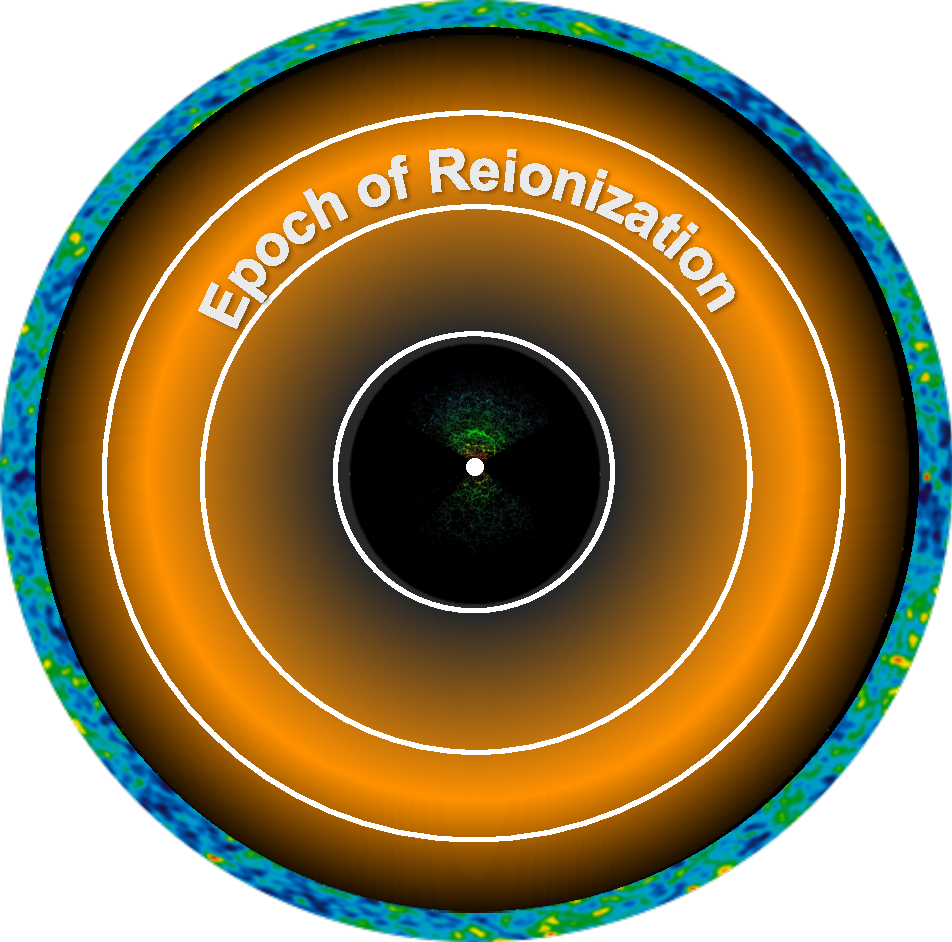
\includegraphics[width=0.5\textwidth]{plots/timeline_circle.pdf}
	\caption{A cartoon diagram of the observable Universe, centered on us. Close-by, galaxy observations have mapped out cosmic web structure in our nearby Universe (image credit: SDSS). Far-away, the cosmic microwave background is observed at a redshift of $z \sim 1100$ (image credit: WMAP). The Epoch of Reionization represents a largely unexplored era between the two, and can be probed by measuring red-shifted $21$\,cm radiation from neutral hydrogen.}
	\label{fig:timeline_circle}
\end{figure}

\begin{figure}
	\centering
	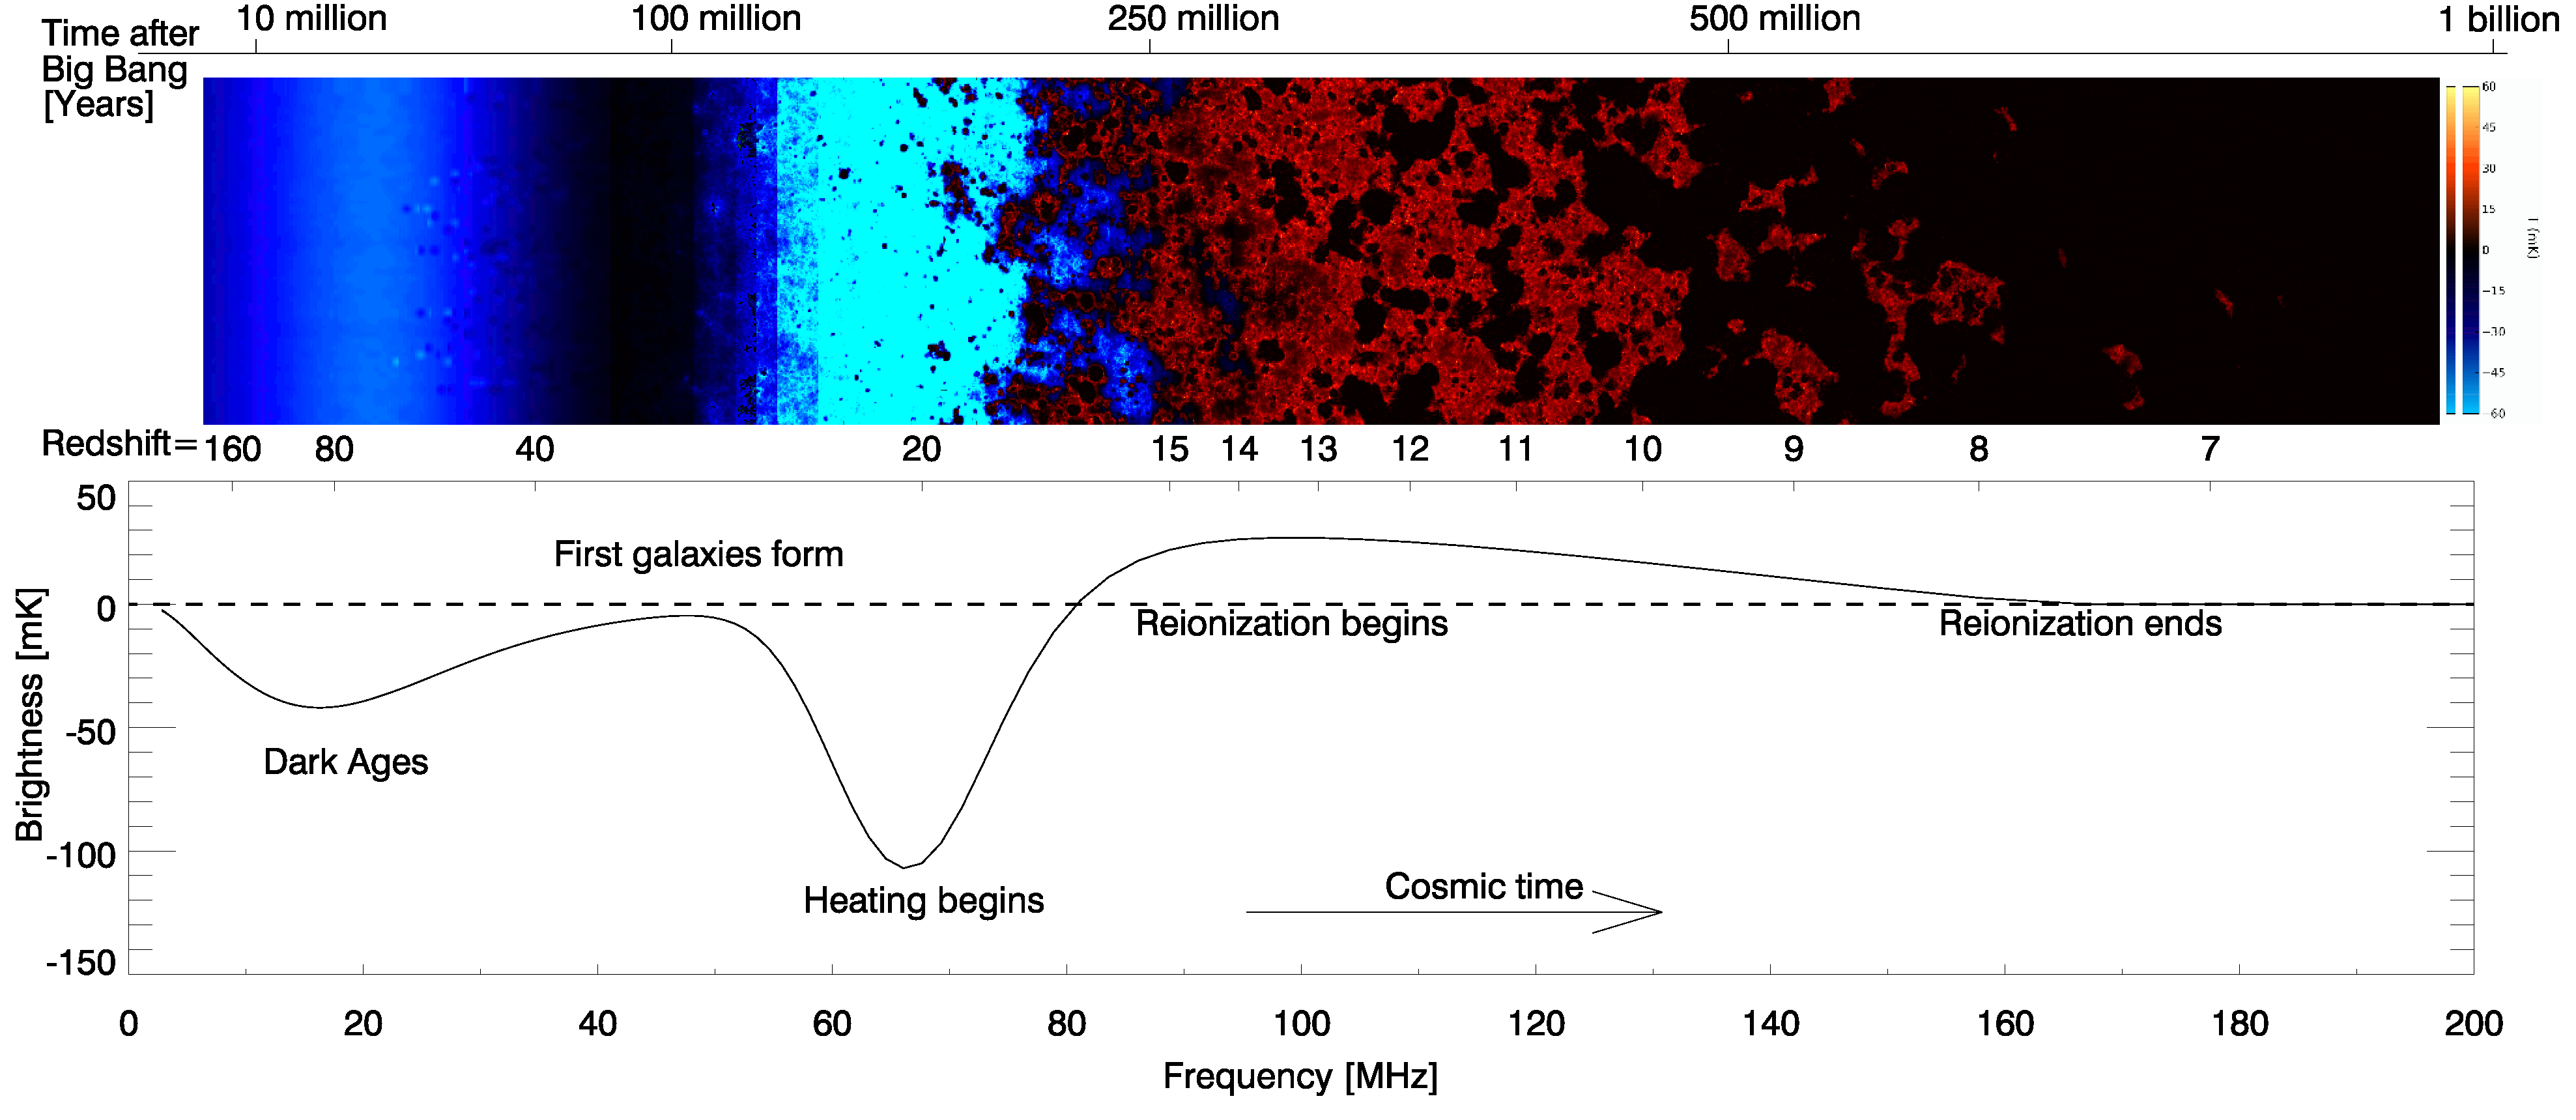
\includegraphics[width=\columnwidth]{plots/timeline_global.pdf}
	\caption{The evolution of the global $21$\,cm signal, starting with the Dark Ages, through galaxy formation and reionization (image credit: \citet{pritchard_loeb2012}). The work in this thesis mainly focuses on a redshift range of $6 < z < 12$ when reionization is expected to progress and complete.}
	\label{fig:timeline_global}
\end{figure}

In practice, the $21$\,cm signal is encapsulated by the quantity $T_{\rm spin}$ (spin temperature), which measures the relative number of hydrogen atoms in the excited (aligned) versus ground (anti-aligned) spin-flip state. A high spin temperature means that the hydrogen gas is more likely to emit $21$\,cm photons, whereas a low $T_{\rm spin}$ implies that the gas is more likely to absorb $21$\,cm photons. 

The spin temperature is always measured with respect to the temperature of the CMB ($T_{\rm CMB}$), which serves as a backlight for our measurement. During different stages of our cosmic history, $T_{\rm CMB}$ and $T_{\rm spin}$ take turns in the spotlight, with the \textit{differential brightness temperature} $\delta T_{b}$ describing their evolution:

\begin{equation}
\label{eq:Tb}
\delta T_{b} \propto (1+\delta_{b})x_{HI}\Big(1-\frac{T_{\rm CMB}}{T_{\rm spin}}\Big).
\end{equation}
Equation \eqref{eq:Tb} captures the EoR signal that $21$\,cm experiments seek to measure, where $\delta_{b}$ is the fractional over-density of matter and $x_{HI}$ is the fraction of neutral hydrogen ($1$ if all neutral, $0$ if all ionized). The differential brightness temperature can be measured in multiple ways --- in Chapter \ref{sec:interferometry} we explain how interferometry (multiple telescopes) can be used to measure the correlations of $\delta T_{b}$ on various spatial scales on the sky. Here we describe the evolution of the sky-averaged $\delta T_{b}$, called the \textit{global signal}, in order to summarize how it is expected to behave during our cosmic dawn and through reionization.

A theoretical prediction for the evolution of $\delta T_{b}$ is shown in Figure \ref{fig:timeline_global}. At the very far left, a cool, neutral IGM remains after recombination and the release of the CMB. Residual electrons collide off of both CMB photons and the hydrogen gas, driving couplings between $T_{\rm gas}$ and $T_{\rm CMB}$, and $T_{\rm gas}$ and $T_{\rm spin}$, respectively. Hence, we expect to see no signal ($\delta T_{b} = 0$) at this time.

During the Dark Ages, collisions still couple $T_{\rm gas}$ and $T_{\rm spin}$, but Compton scattering becomes rarer as the CMB dilutes with the expansion of the Universe. While the CMB dilutes as $T_{\rm CMB} \propto 1/a$, where $a$ is the scale factor, the gas now follows an adiabatic expansion ($T_{\rm gas} \propto 1/a^{2}$). Thus, the gas cools quicker than the CMB, and since it is still coupled to the spin temperature, $T_{\rm spin} < T_{\rm CMB}$ and the signal is expected to be seen in absorption. By the time the first galaxies begin forming, however, the gas is expected to be so dilute that it is no longer coupled to the spin temperature. The spin temperature therefore couples once again to the CMB, and no signal is produced.

As the first stars in the first galaxies begin emitting Lyman-$\alpha$ photons, they are resonantly scattered off of hydrogen via the Wouthuysen-Field effect (the absorption and emission of Lyman-$\alpha$ photons redistributes the spin-flip states), coupling $T_{\rm spin}$ and $T_{\rm gas}$ (\citealt{pritchard_and_loeb2010}). The gas, still cool from adiabatic expansion, implies that $T_{\rm spin} < T_{\rm CMB}$ and the signal is seen in absorption. Eventually, due to their long mean free paths, x-rays from the first sources are thought to be the primary drivers behind heating of the cooled, low-density gas (\citealt{furlanetto_et_al2006}). This drives both the gas and spin temperatures above that of the CMB, where the signal is expected to be seen in emission for the first time. 

Finally, even though the timing and details of reionization are unknown, UV photons from the first luminous structures are believed to eventually ionize all the neutral hydrogen, leaving no signal to be detected by a redshift of $z \sim 6$. 

The shape of the global signal holds important science implications about our early Universe. For example, the timing of the heating trough reveals the types of sources responsible for heating (i.e., late heating implies harder x-ray spectras for x-ray binaries, as shown in \citet{fialkov_et_al2014}). It also contains information regarding the sizes of the dark matter halos hosting those first sources and the cooling mechanisms responsible for star formation (\citealt{fialkov_et_al2014b}). The shape of the absorption feature is also dependent on a number of factors, such as x-ray and Lyman-$\alpha$ emissivities, which in turn are dependent on the nature of the first sources and properties of star formation. For high Lyman-$\alpha$ production rates, a deep trough would be present due to strong couplings between $T_{\rm spin}$ and $T_{\rm gas}$ as the gas cools. An even more pronounced absorption signature, such as the first tentative detection from the Experiment to Detect the Global Epoch of Reionization Signature (EDGES), requires additional physical explanations beyond known physics and commonly accepted scenarios (\citealt{bowman_et_al2018}). 

If the global signal's primary absorption feature unlocks clues about the first sources, the reionization peak and its subsequent decay hold the key for understanding the evolution of the neutral fraction $x_{HI}$. Namely, a direct measurement of $\delta T_{b}$ during this time would shed light about the duration and rate of the reionization process, which in turn can be translated into an evolution for $x_{HI}$. A long reionization duration, for example, would yield a slowly varying neutral fraction evolution, while a more instantaneous reionization would produce a sharp drop-off feature (\citealt{pritchard_and_loeb2010}). One thing is for certain though --- as the field continues to investigate our cosmic dawn and the EoR through HI measurements (both the global signal and statistical fluctuations), we can expect to learn much about the constituents that make up the Universe and their complex interactions during this era.

\subsection{This Thesis}

Although $21$\,cm observations promises an uninterrupted window into the EoR, from which we can learn much about galaxy formation and the properties of the IGM, there are many challenges facing this field of cosmology. In general, the $21$\,cm signal is extremely faint, with bright foregrounds (mostly synchrotron radiation from our own Galaxy) and radio interference easily overshadowing the target signal. As a consequence, instruments need to be extremely well-understood, precisely calibrated, and sensitive enough for a successful detection. In addition, analysis techniques must be innovative and rigorously construed so as to be able to extract clean and accurate measurements.

In this thesis, I present work associated with data from radio interferometers seeking to measure $21$\,cm fluctuations during the EoR. While a confirmed detection by an interferometer remains elusive at this time, this work serves as a huge leap forward in working with large datasets and extracting measurements of the cosmological signal with confidence. The rest of this thesis thus focuses on the characterization of data from large telescope arrays in order to place accurate, stringent limits on the EoR signal. This field is still young, and the work in this thesis serves as a foundation of what promises to be an eye-opening adventure to-come.

\section{Interferometry}
\label{sec:interferometry}

Multiple radio telescopes (i.e., an interferometer) can be used in combination to probe $21$\,cm fluctuations. Rather than a single element, or aperture, many antennas can be used to increase the effective aperture size of the telescope.

As a simplistic example, two antennas may observe the same sky but each receives the sky signal at slightly different times, with a time delay determined by the antenna spacing, or baseline orientation and length, with respect to the sky. The two voltage streams from the antennas can then be correlated to form an output response with an amplitude dependent on the sky's intensity and a phase dependent on the time delay between the two elements and the frequency of the light. The power received by this baseline, as we will see, represents one sample in the large ``synthesized" aperture of the interferometer. Knowledge of the entire sky can be built up by having a large number of antennas and many different types, and copies, of baselines.

\subsection{The Visibility Equation}

The output measurement from correlating signals between two antennas is called a \textit{visibility}. The visibility can be written as:

\begin{equation}
\label{eq:vis}
V_{ij}(\nu) = S(\nu) e^{-2\pi i\frac{\vec{b}_{ij}\cdot \hat{s}}{\lambda}},
\end{equation}
where $i$ and $j$ represent a pair of antennas, $S(\nu)$ is the sky flux density, $\vec{b}_{ij}$ is the baseline vector, $\hat{s}$ is a unit-vector in the direction of a source in the sky, and $\lambda$ is the wavelength of the signal. The fractional term in the exponential reflects the changing number of wavelengths between the two antennas as a signal goes in and out of phase as the source passes overhead. The entire exponential term represents the phase of the visibility, which can also be described as the fringe pattern, or diffraction, or interference pattern, between two antenna elements. 

Equation \eqref{eq:vis} represents a visibility measurement for one direction on the sky. In practice, we compute the integrated visibility over the entire angular sky $d\Omega$:

\begin{equation}
V_{ij}(\nu,\Omega) = \int A(\nu,\Omega)I(\nu,\Omega) e^{-2\pi i\frac{\vec{b}_{ij}\cdot \hat{s}(\Omega)}{\lambda}}d\Omega,
\end{equation}
where the amplitude component has been broken up into a primary beam component $A(\nu,\Omega)$ and sky intensity component $I(\nu,\Omega)$. The primary beam describes the power pattern of an antenna element and determines its field of view. The total power received by an antenna can therefore be thought of as a combination of the intensity distribution on the sky and how receptive the antenna is, or more specifically, the convolution between the two terms (\citealt{thompson_et_al2001}).

The visibility equation can be re-interpreted as the 2-dimensional Fourier-transform of the sky, or a sample of the \textit{uv}-plane, where $u$ and $v$ are sine-waves in a 2D image. In other words, every baseline measures a different Fourier-mode of the sky. To form an image, the Fourier-transform of a visibility would produce a \textit{dirty image} of the sky, from which the true sky can be reconstructed by de-convolving out information from the antenna beam. In this thesis, however, we focus on the 3D Fourier-transform of the sky, or the power spectrum (Chapter \ref{sec:PSoverview}), instead of making images. Hence, we work directly with visibilities as a starting point, which has already taken two Fourier-transforms for us. 

\subsection{The $21$\,cm Power Spectrum}
\label{sec:PSoverview}

In this thesis, we focus on cross-correlations, or power spectral measurements, of visibilities. Recalling that we seek to measure the differential brightness temperature on various spatial scales of the sky, we can form the quantity:

\begin{equation}
\label{eq:PSdef}
\langle \delta \tilde{T}_{b}(\vec{k})^{\ast} \delta \tilde{T}_{b}(\vec{k})\rangle = (2\pi)^{3} \delta^{D}(\vec{k}-\vec{k}')P_{21}(\vec{k}) ,
\end{equation}
where $\delta \tilde{T}_{b}(\vec{k})$ is the Fourier-transform of the differential sky brightness as a function of cosmological wavenumber $\vec{k}$ (i.e., our visibility measurement, up to scaling factors), $\delta^{D}$ is the Dirac-delta function, and $P_{21}$ is the $21$\,cm power spectrum quantity we are interested in eventually forming.

Simply speaking, because our visibility measurements have already taken two spatial Fourier-transforms out of the three needed for a 3D power spectrum, we need only to take one last Fourier-transform (along frequency), and then multiply and average the visibilities together for a given baseline in order to compute a power spectral measurement. Having repeated baseline copies then increases the sensitivity to a given Fourier-mode on the sky, while having different types of baselines makes it possible to measure multiple Fourier-modes and build up an image of the sky. Since the EoR signal is expected to be present everywhere on the sky, in this work we focus on the former technique in order to maximize our sensitivity to the cosmological signal.

We note that the wavenumber $\vec{k}$ can be broken up into a perpendicular component $\vec{k}_{\perp}$ and a parallel component $k_{\parallel}$, where $\vec{k}_{\perp}$ is proportional to the (x,y) spatial coordinates on the sky and $k_{\parallel}$ is proportional to the line-of-sight direction on the sky (i.e., frequency). Every unique baseline probes a single $\vec{k}_{\perp}$, and it's worth noting that, because we focus on redundant baselines in the analysis to follow, most of our power spectrum sensitivity comes from the frequency-direction. Accounting for cosmological distance, a 1D wavenumber has units of Mpc$^{-1}$, so that the 3D power spectrum has units of mK$^{2}\cdot$Mpc$^{3}$. Visibility measurements typically have units of Janskys.

Just as the shape of the global signal provides insight about the early Universe, the shape of the cross-power spectrum, as defined by Equation \eqref{eq:PSdef}, also delivers a wealth of information. Figure \ref{fig:PS_evolution} shows the $21$\,cm ``dimensionless" power spectrum $\Delta^{2}(k)$ (units of mK), defined as:

\begin{equation}
\Delta^{2}(k) = \frac{k^{3}}{2\pi^{2}}P_{21}(k),
\end{equation}
as a function of the magnitude of $k$. This figure shows the expected evolution of the power spectrum, where the overall signal moves to small scales (large $k$) as more hydrogen becomes ionized (the large regions of neutral hydrogen turn into smaller and smaller pockets). This effect can be seen by both the steepening of the spectrum as the neutral fraction decreases, and the time-evolution of the spectrum at a specific (large) $k$.

The $21$\,cm power spectrum therefore encodes important information about the spatial and temporal evolution of reionization, and the shape of the spectrum can be directly mapped to sizes of the ionized bubbles as they grow. Additionally, the power spectrum, which is a function of the differential brightness temperature, can be used to constrain both $T_{\rm spin}$ (and $T_{\rm gas}$, since they're coupled during this era) and $x_{HI}$ via Equation \eqref{eq:Tb}. It is thus a powerful tool for unlocking the properties of the IGM.

\begin{figure}
    \centering
    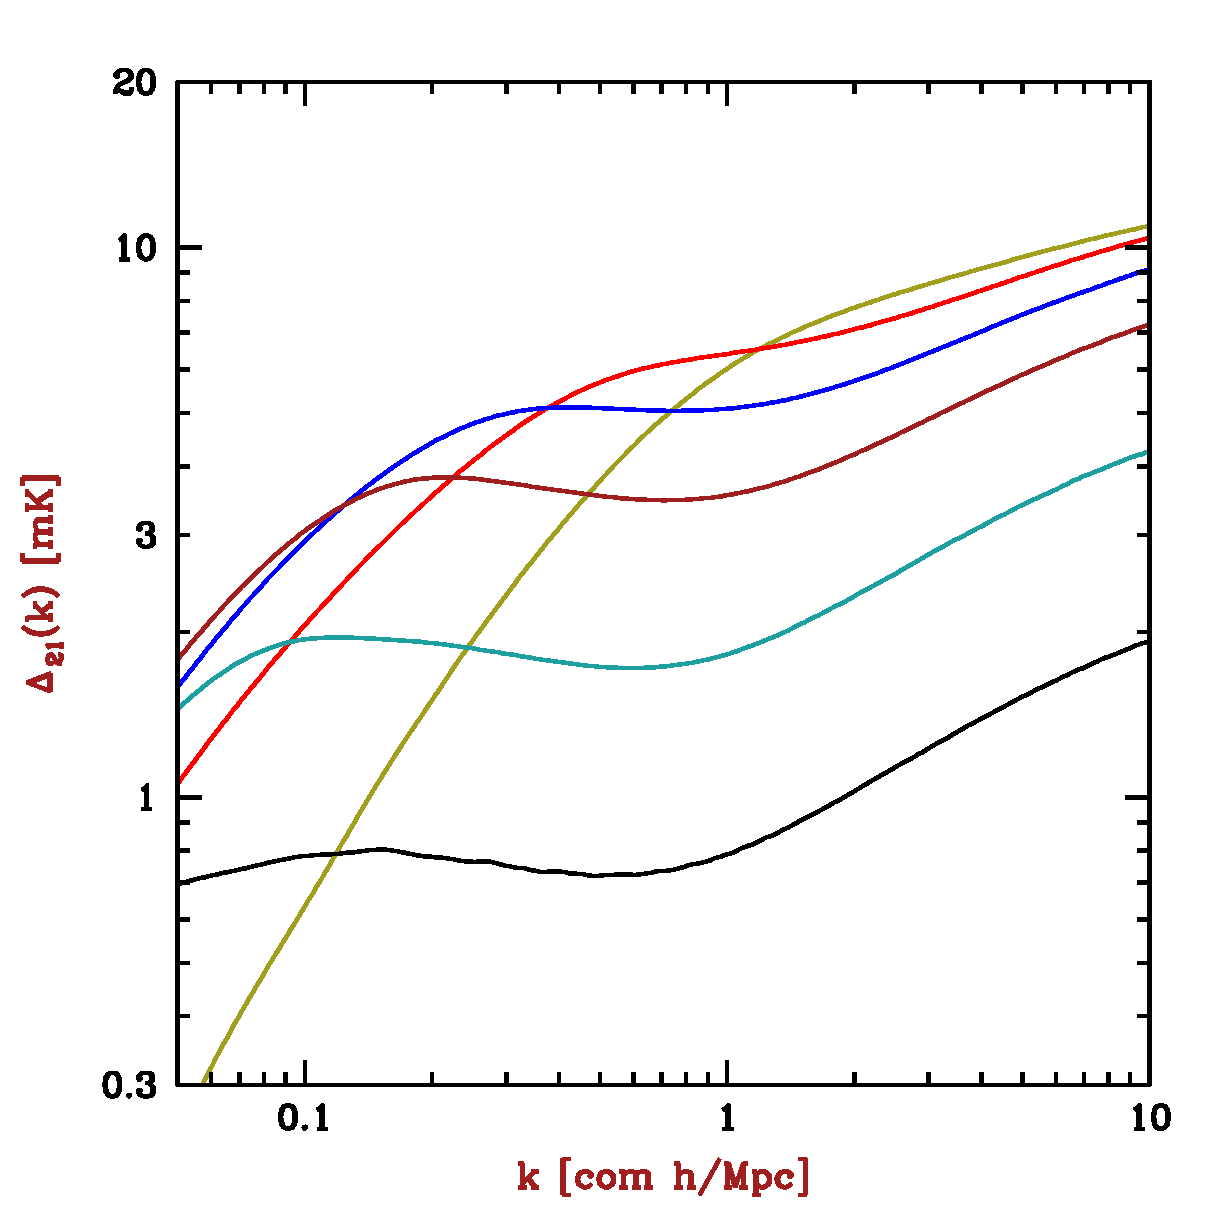
\includegraphics[width=0.45\textwidth]{plots/PS_evolution.eps}
    \caption{The theoretical evolution of the cross-$21$\,cm power spectrum for a specific model (image credit: \citet{barkana2009}), where the neutral fraction $x_{HI} = 10\%$, $30\%$, $50\%$, $70\%$, $90\%$, and $98\%$ from top to bottom at large $k$. This figure shows the expected evolution of the power spectrum which interferometers seek to measure.}
    \label{fig:PS_evolution}
\end{figure}

\subsection{Calibration}
\label{sec:calibration_intro}

We now transition to a brief overview of key data processing steps that are often standard routines when going from visibilities to power spectra. We speak broadly about these steps in this chapter, and go into detail about them for specific experiments in later chapters.

As discussed previously, an interferometer measures a visibility for every baseline pair and every time integration. Repeated baseline types and multi-day observations can be stacked to gain sensitivity to Fourier-modes on the sky. However, ensuring clean measurements at EoR sensitivities requires many other crucial processing steps, including calibration, which we give an overview of in this section.

We've seen that the visibility measurement is dependent on the sky, baseline, and antenna beam, but it is also affected by instrumental systematics. For example, certain components in the signal chain of an instrument can contribute variable noise, losses can arise from reflections, and blockage and scattering may occur. These are all effects that must be considered in order to accurately extract the EoR signal. 

Many of these effects can be mitigated through precise calibration. There are two main types of calibration used by $21$\,cm interferometers: \textit{redundant} calibration and \textit{absolute} calibration. We will briefly describe each here.

Redundant calibration is a type of calibration based on the redundant nature of baselines. For experiments like PAPER and HERA, which have many repeated copies of baselines, redundant calibration can be used to bring all identical baselines into agreement (i.e., it calibrates out deviations between baselines of the same type). This calibration is a powerful technique because it does not use any knowledge of the sky, yet can correct for instrumental-induced gain and phase effects brought on by differences in the signal chain attributable to antennas, cables, and receivers (\citealt{liu_et_al2010}).

Mathematically, the visibility $v_{ij}$ of every baseline can be written as:

\begin{equation}
\label{eq:gains}
v_{ij} = g_{i}^{\ast}g_{j}y_{ij} + n_{ij},
\end{equation}
where $g_{i}$ and $g_{j}$ are the complex gains of each antenna, $y_{ij}$ is the ``true" model visibility for that particular baseline type, and $n_{ij}$ is noise. The goal of redundant calibration is to solve for the gain of each antenna and the ``true" visibility of each baseline type. This can be accomplished by setting up a system of linear equations containing every visibility measurement (the method used by PAPER and HERA is detailed in Chapter \ref{sec:PSA64overview}). If there are more measurements than the sum of the number of unique baselines and antennae, then it is a solvable system. 

The complex gains can be further broken down to be written as $g_{i} = e^{\eta_{i} + i\phi_{i}}$ (\citealt{liu_et_al2010}). In other words, by solving for the gains, we are solving for both an amplitude component and a phase offset for each antenna. The gains can then be divided out of every visibility measurement, producing redundantly-calibrated measurements across the whole array.

While redundant calibration is a clever technique for the internal calibration of an interferometer, the calibrated visibility measurements are still on an arbitrary gain scale that has not been matched up to the sky. Hence, absolute calibration refers to using sources in the sky of known brightness (or sky models) in order to solve for the two remaining internal degrees of freedom: an overall gain and an overall phase. Interferometers typically use a standard self-calibration routine to accomplish this, where $y_{ij}$ is known for specific sky sources.

Ultimately, calibration is a crucial step in preparing interferometric data for a power spectrum analysis. A precisely-calibrated instrument will result in cleaner data from which the EoR signal can be accessed.

\subsection{Foreground Filtering}
\label{sec:fg_intro}

Arguably the largest challenge of processing $21$\,cm data is in removing bright foregrounds. There are several techniques to do this, which fall into two main categories: foreground subtraction and foreground avoidance. The former consists of modeling and subtracting out foreground sources, while the latter involves making EoR measurements in a domain where foregrounds are minimal. 

For interferometers with imaging capabilities, foreground removal techniques include modeling approaches to spatially localize and remove contaminants (e.g., \citealt{santos_et_al2005}; \citealt{wang_et_al2006}; \citealt{jelic_et_al2008}; \citealt{liu_et_al2009}; \citealt{bowman_et_al2009}; \citealt{harker_et_al2009}; \citealt{chapman_et_al2016}). This can be done by fitting polynomials to data or by using non-parametric methods, which make fewer assumptions about the form of the foregrounds. While foreground subtraction would be ideal if done accurately, modeling is difficult and subtraction poses the risk of cosmological signal loss.

The other method commonly used, foreground avoidance, is a strategy employed by both PAPER and HERA. Foreground avoidance was originally suggested as an alternate method to the subtraction method, which has stringent requirements in order to yield uncontaminated results. In order to understand foreground avoidance, we must first define the ``EoR Window".

A 3D power spectrum can be split into two directions along $k_{\perp}$ and $k_{\parallel}$, which correspond to modes perpendicular to the line-of-sight and along the line-of-sight, respectively. In this two-dimensional space, there are two main regions --- one relatively free of foregrounds (the ``EoR Window") and one contaminated by foregrounds (the ``wedge"), as shown in Figure \ref{fig:wedge} (e.g., \citealt{datta_et_al2010}; \citealt{vedantham_et_al2012}). We can see this by thinking of the $k_{\parallel}$ direction to be akin to the physical time delay associated with light hitting two antennas (a good approximation, especially for short baselines). As $k_{\perp}$, which is proportional to baseline length, increases, the maximum time delay also increases because it is set by the length of the baseline (i.e., a maximum delay occurs when a source is at the horizon; therefore, the time delay is simply the time it takes for the light to travel the distance of the baseline). Hence, the ``wedge" is formed, representing a region where smooth-spectrum foregrounds are expected to be contained. Said differently, foregrounds are expected to be bound by the light-crossing time between two antennas, and therefore there is a maximum limit for $k_{\parallel}$ (time delay) given a $k_{\perp}$ (baseline). 

Delay-filtering is the process by which foregrounds within the wedge are filtered out, leaving a relatively clean window behind from which the cosmological signal can be extracted (\citealt{parsons_et_al2012b}). This approach limits the number of modes for which the measurement can be made and can suffer from some foreground leakage as explained in Chapter \ref{sec:BiasOverview}, but its advantages include its simplicity and conservativeness (i.e., it leaves all the cosmological signal within the window in tact).

\begin{figure}
    \centering
    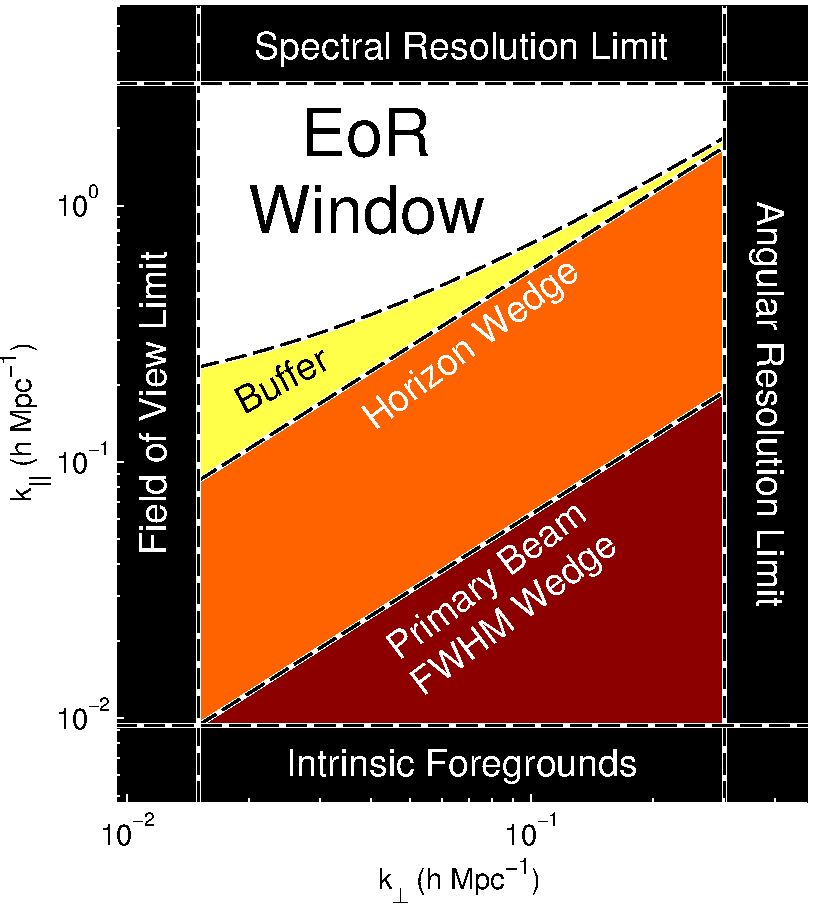
\includegraphics[width=0.45\textwidth]{plots/wedge.pdf}
    \caption{A cartoon diagram of the ``EoR Window" and ``wedge" of foreground contamination in Fourier space (image credit: \citet{dillon_et_al2015b}). A foreground avoidance approach makes power spectrum measurements in the window, while a foreground subtraction approach subtracts out foregrounds so that measurements can be made in the wedge. The overall power spectrum measurement space is limited by an interferometer's field of view and angular resolution along the horizontal axis, and spectral resolution and intrinsic foregrounds along the vertical axis.}
    \label{fig:wedge}
\end{figure}

Whether it's avoidance or removal, there have been many approaches at tackling the challenge of foregrounds (summarized in \citet{chapman_et_al2016}). But, regardless of the method used, removing Galactic and extragalactic foregrounds from $21$\,cm data is absolutely a critical step for analyses seeking the EoR signal. 

\subsection{Fringe-rate Filtering}
\label{sec:frf_intro}

The final analysis technique to introduce in this section is fringe-rate filtering, a filtering scheme carried out in a domain which is the Fourier-dual to time. This type of filtering aims to optimize the process of combining time-ordered data and has been investigated in \citet{roshi_perley2003}, \citet{parsons_backer2009}, \citet{offringa_et_al2012}, and \citet{parsons_et_al2016}.

A ``fringe-rate" is the rate at which the sky moves relative to the fringe pattern of an interferometer. As sources pass overhead, they walk in and out of the interference pattern of two antennas, and the rate at which this movement happens is dependent on the source's declination and hour angle. For example, a source located near a celestial pole has a zero fringe-rate, as it does not appear to move in the sky as the Earth rotates. However, a source located on the celestial equator will have a maximum fringe-rate set by the rate of Earth's rotation. The sky can therefore be decomposed into fringe-rate bins, each of which forms a concentric circle of constant fringe-rate around the celestial sphere.

One initial advantage of filtering in fringe-rate space is that it allows the filtering of noise that is not associated with movement locked on the sky (i.e., filtering out fringe-rates greater than the maximum allowed by the Earth's rotation). This excess noise can come from the instrument itself or from signals with an origin not on the sky. Additionally, one can up-weight and down-weight certain portions of the sky by choosing different linear combinations of fringe-rates (\citealt{parsons_et_al2016}). This allows what is effectively a beam-sculpting operation, where the most sensitive parts of one's beam can be up-weighted compared to others.

A third advantage of this type of filtering is that it can also be used to integrate visibilities in time. Depending on the shape of the filter in the fringe-rate domain, the effect in the time domain can be an averaging operation along time. This is advantageous because it allows an optimal way of combining measurements (by weighting fringe-rates differently based on signal-to-noise ratios in each fringe-rate bin, for example) compared to a more traditional boxcar average, which does not use information from individual fringe-rate bins.

Broadly, fringe-rate filtering can be thought of as a tailored filtering step that can increase the sensitivity of a measurement by differentiating between noise- and signal-like modes in data. When carefully chosen, a fringe-rate filter can enhance modes containing emission from the celestial sphere, where the $21$\,cm signal lies.

\section{Instruments}

The recent exploration of our cosmic dawn has led to the development of multiple experiments that are aiming to detect the $21$\,cm signal from neutral hydrogen during reionization. In this section we will first highlight the two main radio interferometers whose data is used in this thesis, and then discuss other similar experiments along with the current status of the field.

\subsection{The Precision Array for Probing the Epoch of Reionization}
\label{sec:PAPER_intro}

The Precision Array for Probing the Epoch of Reionization (PAPER) is a first generation EoR experiment. Its history dates back to 2007, when an initial four dipole antennas observed the sky from Western Australia. A year later, the array increased to eight stations and moved to Green Bank, West Virginia. These first two deployments are summarized in \citet{parsons_et_al2010} and were used to characterize important aspects of the instrument, including system performance, beam models, instrumental temperatures, and sensitivity to radio frequency interference (RFI). 

PAPER then moved to the Karoo Desert in South Africa, near the Square Kilometre Array South Africa (SKA-SA). The PAPER array doubled in size each year, starting with 32 antennas in 2011 and ending with 128 a few years later. PAPER's observing seasons using these three arrays (PAPER-32, PAPER-64, and PAPER-128) have primarily been used to develop analysis techniques, understand instrumental design, and begin to place limits on the EoR and connect them to science implications.

A brief overview of the PAPER instrument and digital backend follows. The PAPER dipole itself (Figure \ref{fig:paper_dipole}) is made from two rods of copper sandwiched between two aluminum disks. The sizes of each are fine-tuned to produce an antenna frequency response between 100-200\,MHz. Each PAPER antenna is sensitive to two orthogonal polarizations, those being the East/West and North/South directions (XX and YY linear polarizations) given the antenna's orientation on the ground. A grounding structure, made of wire-mesh and held in place by PVC pipes, is both underneath the dipole and surrounds it as four angled panels. The design of the antenna's framework was driven by the desire to produce spectrally and spatially smooth beam responses as discussed in \citet{parsons_et_al2010} and \citet{pober_et_al2012}. Altogether, an entire PAPER dipole measures about 2\,m on each side and sits still while the Earth's rotation moves the sky above (``drift-scan" mode). When photons hit the dipoles' copper rods, electrons are excited and their movement turns the electric field into a voltage that can be measured.

\begin{figure}
    \centering
    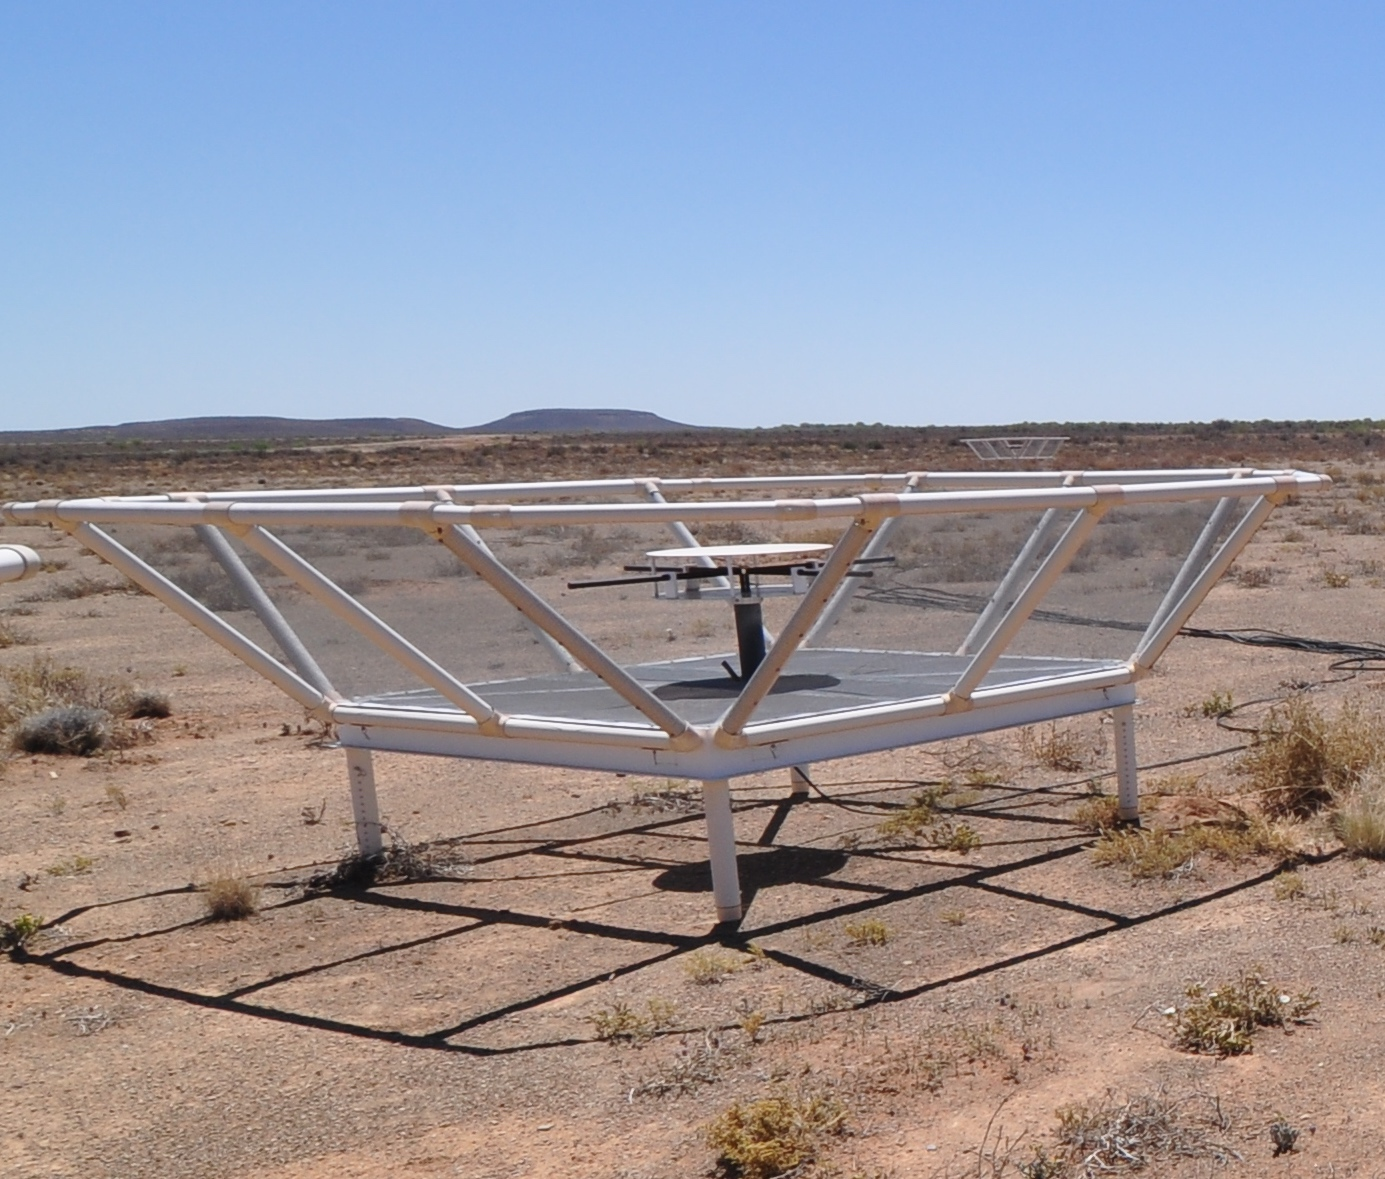
\includegraphics[width=0.5\textwidth]{plots/paper_dipole2.jpg}
    \caption{A PAPER antenna in the Karoo Desert in South Africa. A dual-polarization dipole sits at the center, surrounded by wire mesh panels that measure 2\,m on each side.}
    \label{fig:paper_dipole}
\end{figure}

In short, PAPER's analog system consists of a balun attached to each dipole element (which measures the voltage and amplifies the signal) and coaxial cables which transport the antenna signals. The signals then travel to dual-channel receiver boards which are cooled inside thermal enclosures in order to prevent the introduction of high gains from temperature fluctuations. The receivers both amplify and filter (in frequency) the signals before sending them to the digital system. 

PAPER's digital system is housed inside a refrigerated container on the observing site. The bulk of the processing is carried out by a series of real-time digital FX correlators which cross-correlate pairs of antenna signals to form visibility measurements. More specifically, the FX correlators comprise of ``F-engines" which digitize, down-convert, and channelize antenna inputs, a switch that divides the data into frequency subsets and routes the packets, GPUs which cross-multiply signals from all antenna pairs and integrate in time (``X-engines"), and finally another switch and computer which collect the data, writes it to disk, and sends the final products over an ethernet connection as ``raw" visibility data products that are ready to be analyzed. 

Much of PAPER's digital signal processing (DSP) system has been made possible due to the development of hardware by the Center for Astronomy Signal Processing and Electronics Research (CAPSER). We rely on their Field-programmable Gate Array (FPGA) processors which can quickly perform the fast Fourier-transforms required to produce visibilities. The development of FPGA's into PAPER's DSP system has been critical in allowing for the scalable expansion of the array. 

PAPER's first power spectrum limits on the EoR came from its 32-element array (\citealt{parsons_et_al2014}). PAPER-32 observed in a redundantly-configured layout from 2011-2012, producing a published $2\sigma$ upper limit on the $21$\,cm power spectrum of (41\,mK)$^{2}$ for $k=0.27\, h$\,Mpc$^{-1}$ at $z=7.7$ (\citealt{parsons_et_al2014}). This result, while orders of magnitude above predicted EoR signals, was used to generate constraints on the brightness temperature of $21$\,cm emission for various reionization models and rule out cold reionization scenarios (i.e., some heating of the IGM is necessary by $z=7.7$ to be consistent with PAPER-32's results).

PAPER expanded to 64 elements in 2012, keeping its redundant layout in order to maximize power spectrum sensitivity. The analysis and initial results for PAPER-64's observing season is outlined in \citealt{ali_et_al2015}, where a $2\sigma$ upper limit on the EoR is published as (22\,mK)$^{2}$ for $0.15 < k < 0.5\,h$\,Mpc$^{-1}$ at $z=8.4$. A result at this sensitivity can begin to place more interesting limits on IGM heating models and on the temperature of the IGM during this time (\citealt{pober_et_al2015}).

From 2013-2015, PAPER-128 marked the last era for the PAPER experiment. The data collected with this array has not been published publicly and work is ongoing to process and analyze this data. While most of this thesis focuses on PAPER-64, specifically on analysis methods developed to revise the initial (incorrect) PAPER-64 results (Chapter \ref{c.PSmethods}) and what those new limits should be (Chapter \ref{c.PSA64}), we also present a first-look at PAPER-128 and discuss how PAPER's final observing season has influenced analysis metrics for next generation experiment HERA (Chapter \ref{c.PSA128}).

The PAPER experiment as a whole has been absolutely fundamental to the growth of the field of $21$\,cm cosmology. This first generation experiment set a standard for other similar experiments and has provided countless lessons in all aspects of the signal chain. The array may be retired, but its influence will not be forgotten.

\subsection{The Hydrogen Epoch of Reionization Array}

The development of the Hydrogen Epoch of Reionization Array (HERA) was largely driven by the need for increased sensitivity, as even PAPER-128 lacked the collecting area for a significant detection of the EoR. HERA is a second generation EoR experiment currently being built in the Karoo. It features a staged build-out of parabolic dishes with 14\,m diameters, with construction beginning in 2015 and an eventual 350 dishes planned to be completed by the end of 2019.

A HERA dish (Figure \ref{fig:hera_dish}) is made up of wire-mesh, PVC pipes, and wooden support structures. The size, shape, and total number of the dishes were chosen in order to optimize sensitivity (i.e., minimize chromatic effects that would leak power into the EoR window), minimize costs, and be easily scalable and robust for a five year lifetime (\citealt{deboer_et_al2017}). While work on a new feed design (with a wider bandwidth) is ongoing, the first observations from HERA use recycled PAPER dipoles. Suspended upside-down with a wire pulley-system, the PAPER dipoles are surrounded by a wire-mesh backplane structure that minimizes cross-coupling between antennas while optimizing beam efficiency, frequency response, and polarization match (\citealt{deboer_et_al2017}). Similarly, the first stages of the HERA array are using the existing PAPER signal chain and hardware, while work is progressing towards an underground node-based architecture that will house the DSP system and minimize cable reflections by allowing for shorter cable paths. 

\begin{figure}
    \centering
    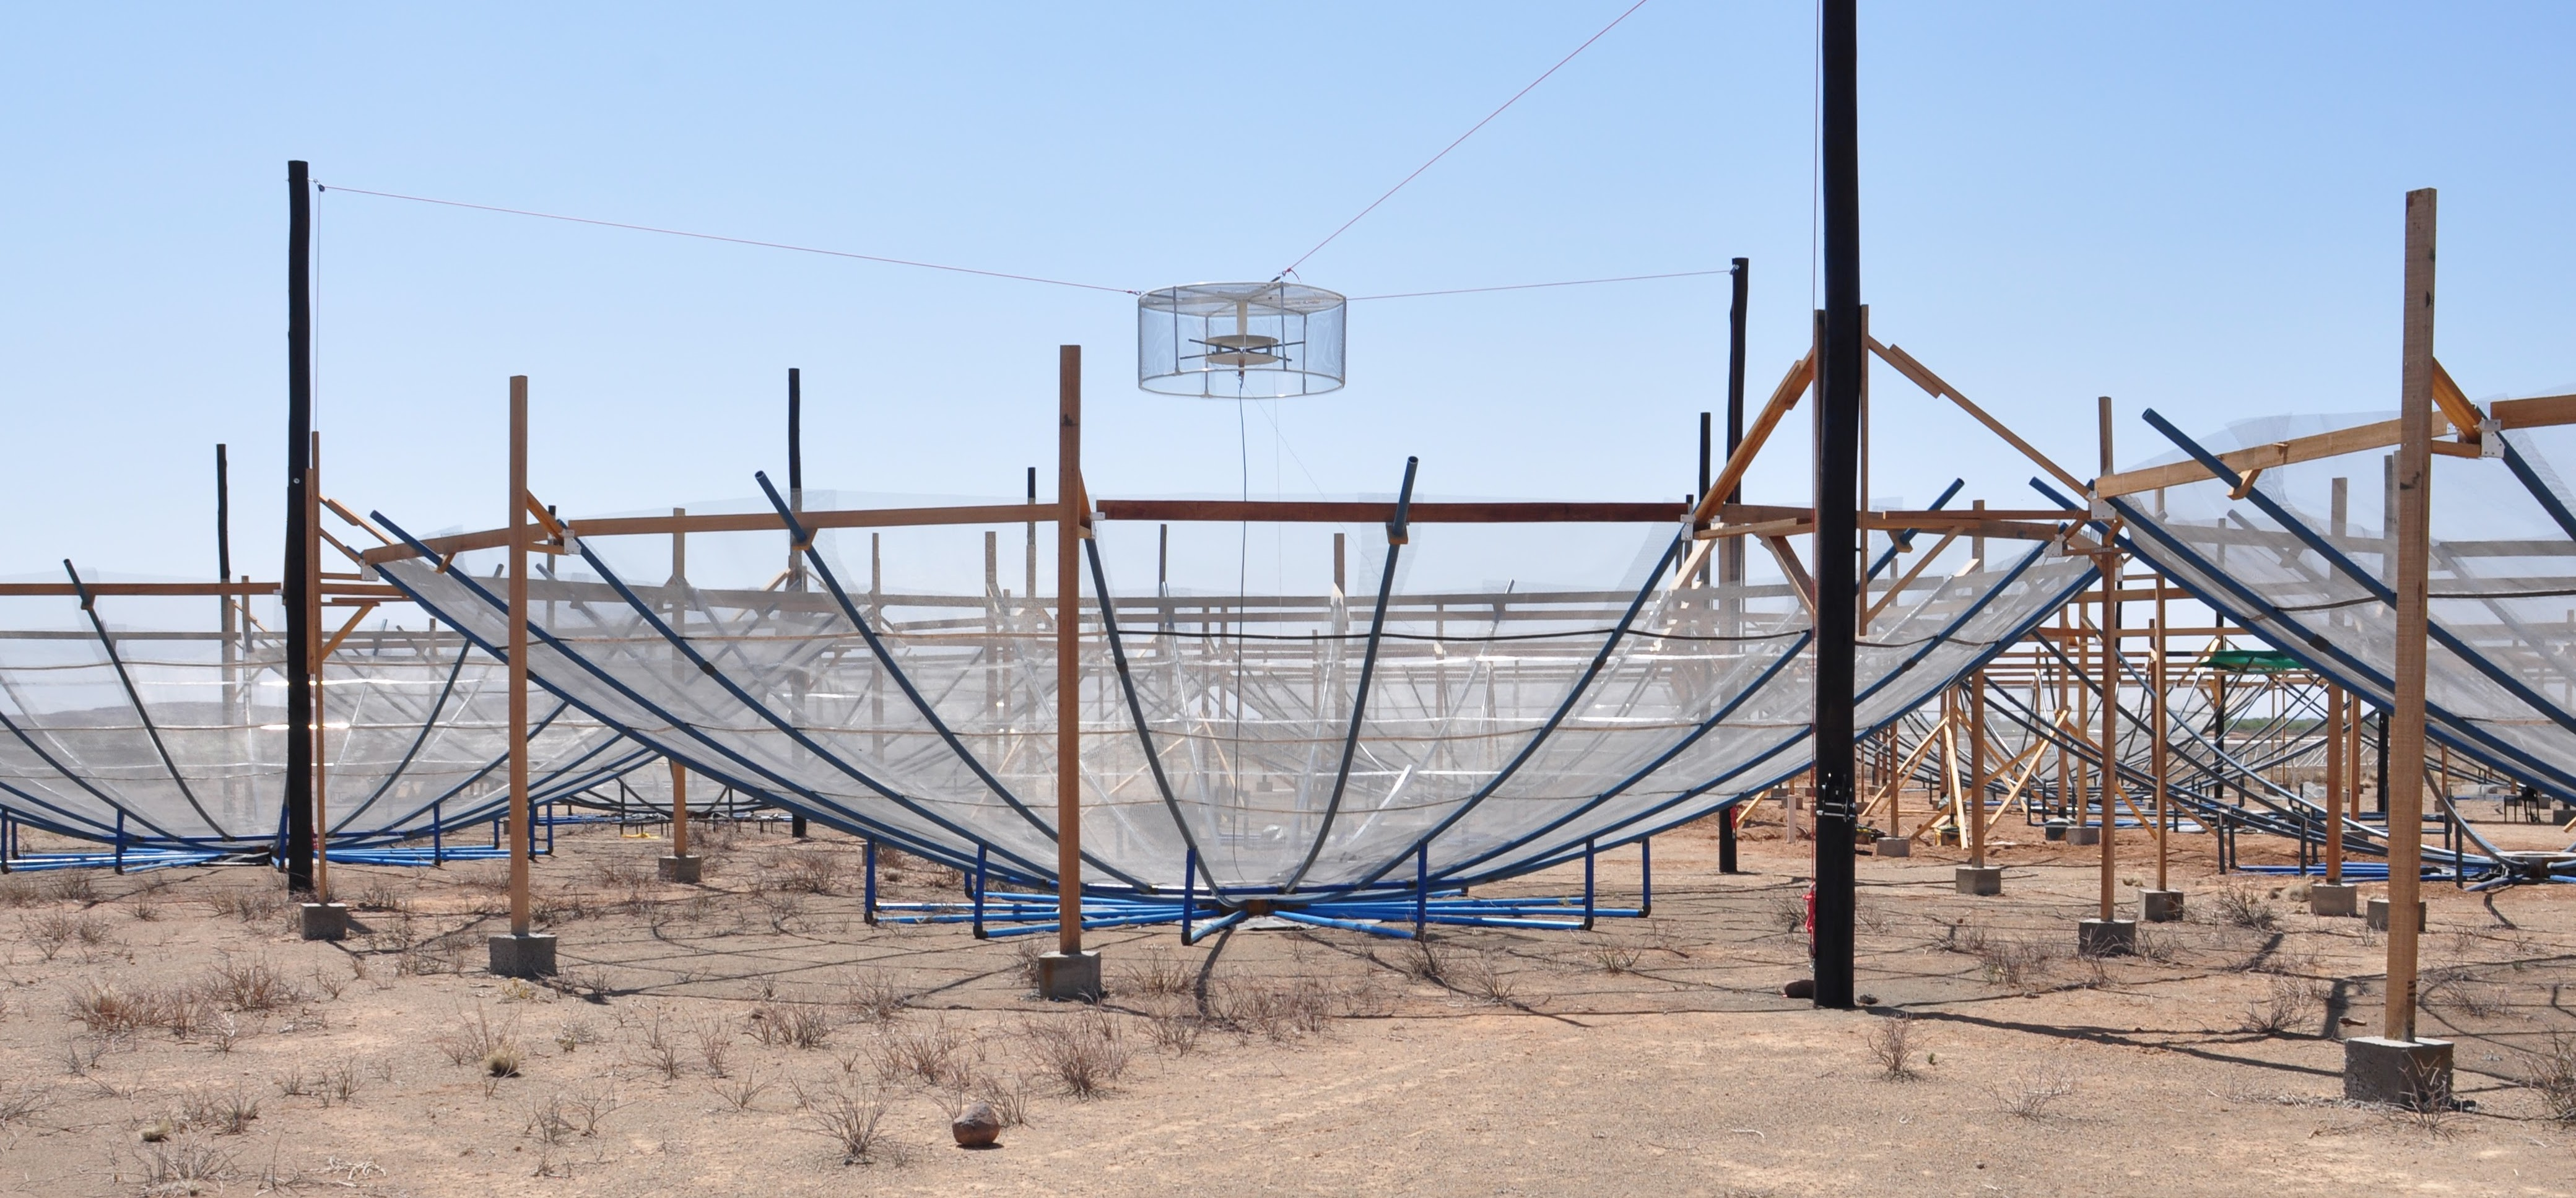
\includegraphics[width=1\textwidth]{plots/hera_dish.jpg}
    \caption{A HERA dish in the Karoo Desert in South Africa. Wire-mesh, PVC pipes, and wooden structures serve as the foundation for the 14\,m diameter parabola. A PAPER dipole is suspended upside-down with a wire pulley-system and surrounded by a prototype wire-mesh skirt structure. HERA-350 will use an updated design for its feed; however, HERA's initial data releases use the old PAPER infrastructure as depicted here.}
    \label{fig:hera_dish}
\end{figure}

The configuration of HERA, like PAPER, is highly redundant and optimized for a robust foreground avoidance approach. Because this power spectrum approach requires short baselines (which minimize the wedge), the HERA antennas are densely-packed next to each other into a main core. This core is segmented into three displaced sections, whose sectioning is designed to improve HERA's imaging ability (\citealt{dillon_parsons2016}). Additionally, there will be 30 outrigger elements joining the full array, allowing for a more complete \textit{uv}-plane coverage and imaging capabilities that can be leveraged for a foreground removal approach. The full HERA array is depicted in Figure \ref{fig:hera_array}. 

\begin{figure}
    \centering
    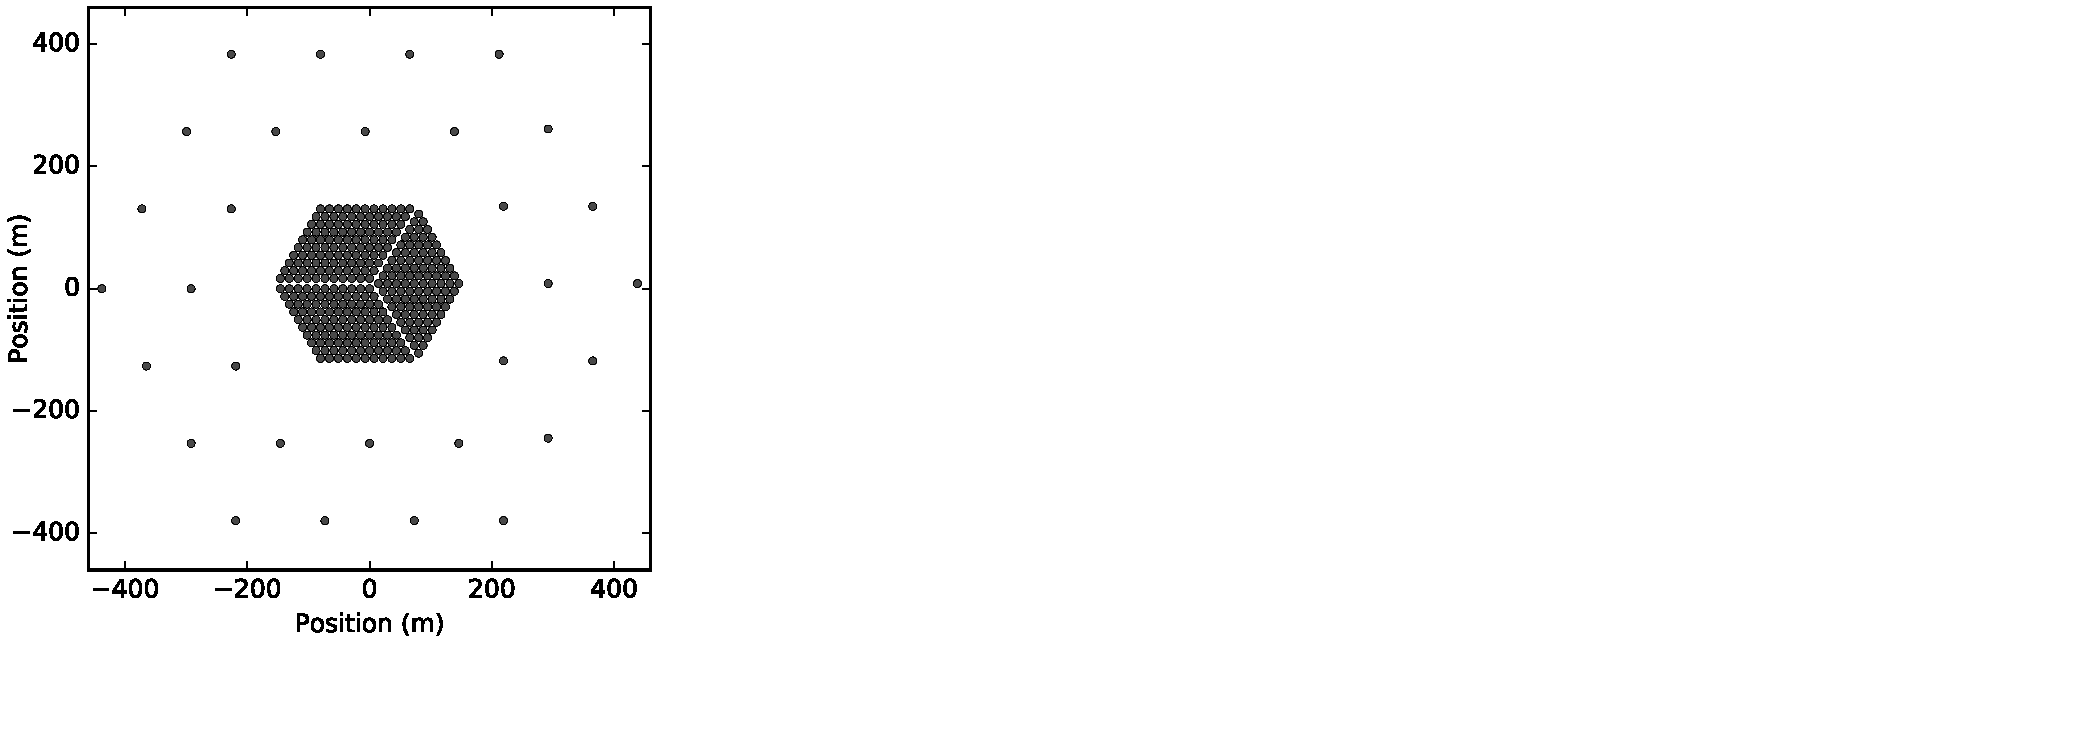
\includegraphics[width=0.5\textwidth]{plots/hera_array.pdf}
    \caption{The full HERA-350 array (image credit: \citet{deboer_et_al2017}). The array is comprised of a segmented densely-packed core (to optimize redundancy for a foreground avoidance approach) and surrounding outrigger elements (for imaging capabilities).}
    \label{fig:hera_array}
\end{figure}

The primary science goal of HERA is to make a high-significance detection of the cosmological signal in order to constrain the timing and morphology of reionization. With precision constraints on the EoR, we can begin to understand the role of the first stars and galaxies in driving reionization, their complex interactions with their environments, and the evolution of cosmic structure. With the full array and an upgraded feed sensitive from 50-250\,MHz, secondary science goals of the instrument include precision cosmology, imaging of the reionization epoch, and an investigation of the pre-reionization heating epoch (\citealt{deboer_et_al2017}). HERA, with a collecting area of $\sim0.1$\,km$^{2}$, is well-poised for these challenges (\citealt{pober_et_al2014}) and has already undergone numerous tests and simulations to ensure that its design meets specification (\citealt{neben_et_al2016}; \citealt{ewall-wice_et_al2017}; \citealt{patra_et_al2018}). As the fully realized HERA soon approaches, there is much to look forward to in the coming years from this array.

\subsection{Other Experiments and Status of Field}

Although this thesis focuses mostly on PAPER data and analysis methods that will be used by HERA, these two arrays are not alone in their quest for the EoR. Other radio interferometers which seek to measure statistical power spectra include the Giant Metre-wave Radio Telescope located in India (GMRT; \citealt{paciga_et_al2013}), the LOw Frequency ARray in Europe (LOFAR; \citealt{van_haarlem_et_al2013}), the Murchison Widefield Array in Australia (MWA; \citealt{tingay_et_al2013}), the 21 Centimeter Array in China (21CMA; \citealt{peterson_et_al2004}; \citealt{wu2009}), and the Square Kilometre Array in South Africa (SKA; \citealt{koopmans_et_al2015}).

Several of these experiments have succeeded in placing upper limits on the EoR, including results from the 32-tile MWA (\citealt{dillon_et_al2014}), 128-tile MWA (\citealt{dillon_et_al2015}; \citealt{beardsley_et_al2016}), GMRT (\citealt{paciga_et_al2013}), and LOFAR (\citealt{patil_et_al2017}). PAPER has also previously published results using 32 antennas (\citealt{parsons_et_al2014}; \citealt{jacobs_et_al2015}) and 64 antennas (\citealt{ali_et_al2015}), though we highlight the errors found in PAPER's analysis pipeline throughout this thesis and thus refer the reader to Chapter \ref{c.PSA64} for updated results from PAPER.

The work in the 21\,cm community that has led to these power spectrum limits (Figure \ref{fig:statusfield}) has largely revolved around the key challenge of controlling foregrounds and systematics. To accomplish this, significant progress has been made in all aspects of the experimental process, ranging from carefully designed interferometers (\citealt{lonsdale_et_al2009}; \citealt{parsons_et_al2012a}; \citealt{dillon_parsons2016}), to novel methods for understanding and dealing with foregrounds (e.g., \citealt{morales_et_al2006}; \citealt{datta_et_al2010}; \citealt{sullivan_et_al2012}; \citealt{moore_et_al2013}; \citealt{hazelton_et_al2013}; \citealt{pober_et_al2013b}; \citealt{liu_et_al2014a}; \citealt{liu_et_al2014b}; \citealt{thyagarajan_et_al2015}), to statistical analysis techniques for precise calibration and power spectrum estimation (e.g., \citealt{liu_et_al2010}; \citealt{trott_et_al2012}; \citealt{liu_et_al2014b}; \citealt{zheng_et_al2014}; \citealt{dillon_et_al2014}; \citealt{jacobs_et_al2016}). PAPER's foreground avoidance strategies have, in particular, led to detailed understandings of redundant calibration and the effects of filtering on the EoR window, while MWA's foreground subtraction techniques have provided complementary improvements in imaging capabilities. While the experiments with published results currently lack the sensitivities needed for an EoR detection, both the delay-filtering and map-making methods, along with hybrid approaches (\citealt{trott_et_al2016}), have set a strong foundation for controlling foregrounds by future, more sensitive interferometers.

Related to the fundamental goal of simultaneously maximizing sensitivity and minimizing contaminants, some other challenges that face current $21$\,cm experiments include polarization leakage from Faraday-rotated emission (\citealt{moore_et_al2013}; \citealt{kohn_et_al2016}; \citealt{nunhokee_et_al2017}), direction-dependent beam effects, and other low level sources of chromaticity induced by the instrument or calibration. These effects will require thorough investigations as experiments approach EoR sensitivities.

\begin{figure}
    \centering
    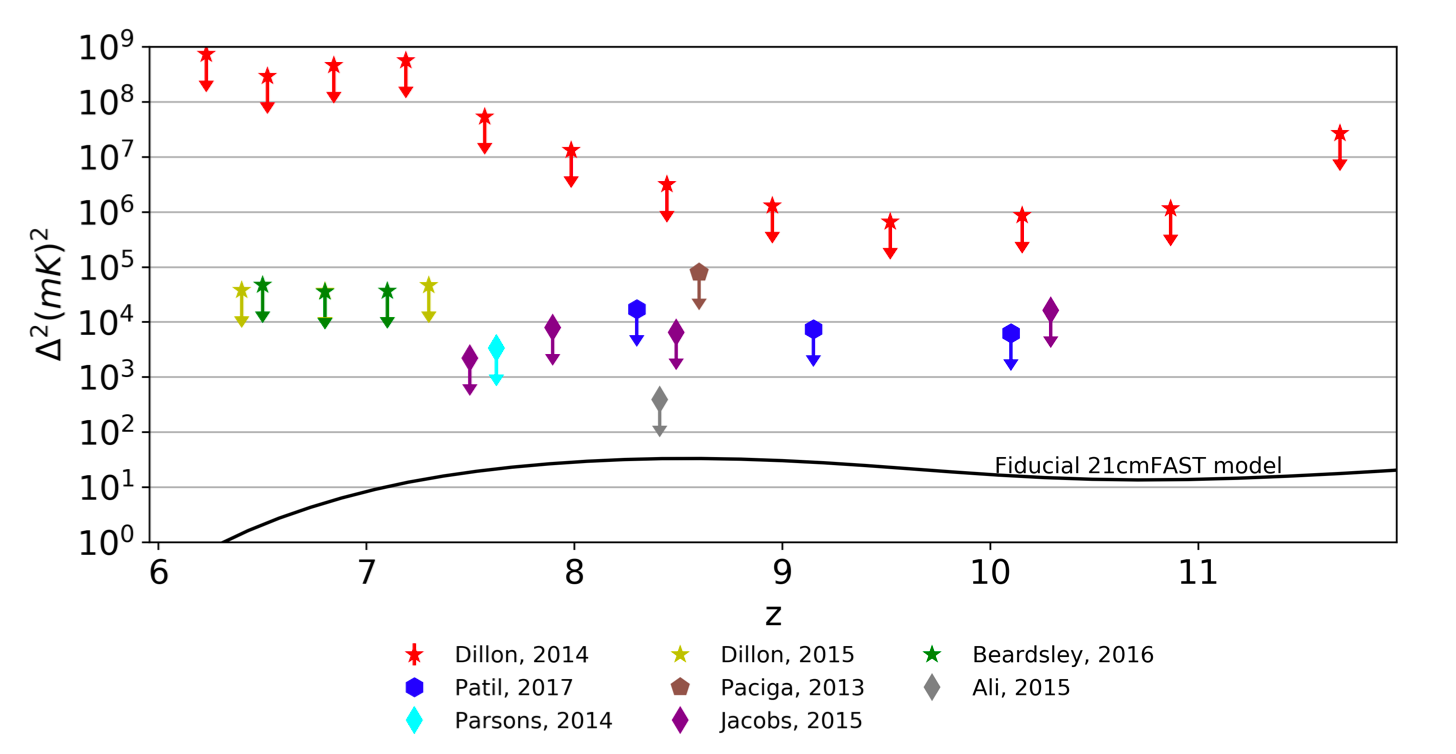
\includegraphics[width=1\textwidth]{plots/statusfield.png}
    \caption{Published upper limits on the EoR placed by different $21$\,cm experiments, prior to the work in this thesis. All PAPER results shown (PAPER-32 is in cyan and magenta, and PAPER-64 is in blue) are suspect to the errors discussed throughout this work and are superseded by the ones presented in Chapter \ref{c.PSA64}.}
    \label{fig:statusfield}
\end{figure}

In addition to power spectrum experiments, there are several complementary experiments that aim to measure the sky-averaged global $21$\,cm signal (i.e., the mean brightness temperature of the EoR relative to the CMB). These include the Experiment to Detect the Global EoR Signature (EDGES; \citealt{bowman2010}), the Large Aperture Experiment to Detect the Dark Ages (LEDA; \citealt{bernardi_et_al2016}), the Dark Ages Radio Explorer (DARE; \citealt{burns2012}), the Sonda Cosmol\'ogica de las Islas para la Detecci\'on de Hidr\'ogeno NeutroSciHi (SCI-HI; \citealt{voytek2014}), the Broadband Instrument for Global HydrOgen ReioNisation Signal (BIGHORNS; \citealt{sokolowski2015}), and the Shaped Antenna measurement of the background RAdio Spectrum (SARAS; \citealt{patra2015}).

Like the power spectrum experiments, global signal experiments also face challenges of bright foregrounds and instrumental systematics. In particular, they require extremely precise calibration in order to avoid overfitting when subtracting foregrounds, and they also face additional challenges when observing the lowest frequencies, such as ionospheric fluctuations and brighter foregrounds (\citealt{vedantham_et_al2014}; \citealt{datta_et_al2014}).

However, most global signal telescopes consist of single elements and can therefore be more easily constructed. Additionally, EoR sensitivities can be reached with relatively short observations. Thus, global signal experiments are actively being worked on as a complementary view into the evolution of the $21$\,cm signal. Accurate detections of the features of the global signal will delineate the different epochs in the early Universe, and their shapes will carry important implications about the nature of the IGM and the first sources.

For example, the first potential detection of the $21$\,cm signal has been made by the global signal experiment EDGES (\citealt{bowman_et_al2018}). This exciting result suggests the presence of an absorption feature in the sky-averaged spectrum at 78\,MHz, thought to be the result of the absorption of CMB photons by HI gas. Because the detected feature is best-fit by an amplitude much larger than what is consistent with expectations for the $21$\,cm signal during this epoch, alternate scientific explanations have been offered, such as the influence of dark matter on baryons and the effect of their interaction on the temperature of the gas (\citealt{barkana2018}; \citealt{slatyer_wu2018}), . Measurements from other experiments in the future will certainly be informative in shaping the community's confidence in this detection, and this result marks just the beginning of many more in the field to come.




